\section{Model Room Illuminance Calculation}
The algorithm was tested on a model room of dimension 10~m $\times$ 5~m $\times$ 4~m. Any barriers or equipment were not taken into account. Pure diffuse reflections were considered with facets' reflectances:

\begin{itemize}
	\item $\rho = 0.2$ for floor,
	\item $\rho = 0.5$ for walls,
	\item $\rho = 0.7$ for ceiling.
\end{itemize}

Each facet was of dimensions 0.25~m $\times$ 0.25~m. 4~reflections were evaluated for each solution, because a higher count of reflections has little to no effect on the overall results. Furthermore each additional reflection slows down calculations significantly. It was found out that there was an increase of less than 10~\% of the resulting illuminance after the 4\textsuperscript{th} reflection. This fact was tested in a simulation with only a single lamp placed in the middle of the room's ceiling. The results are graphically shown in Figure~\ref{fig:reflDif}.

\begin{figure}[htb]
  \centering
  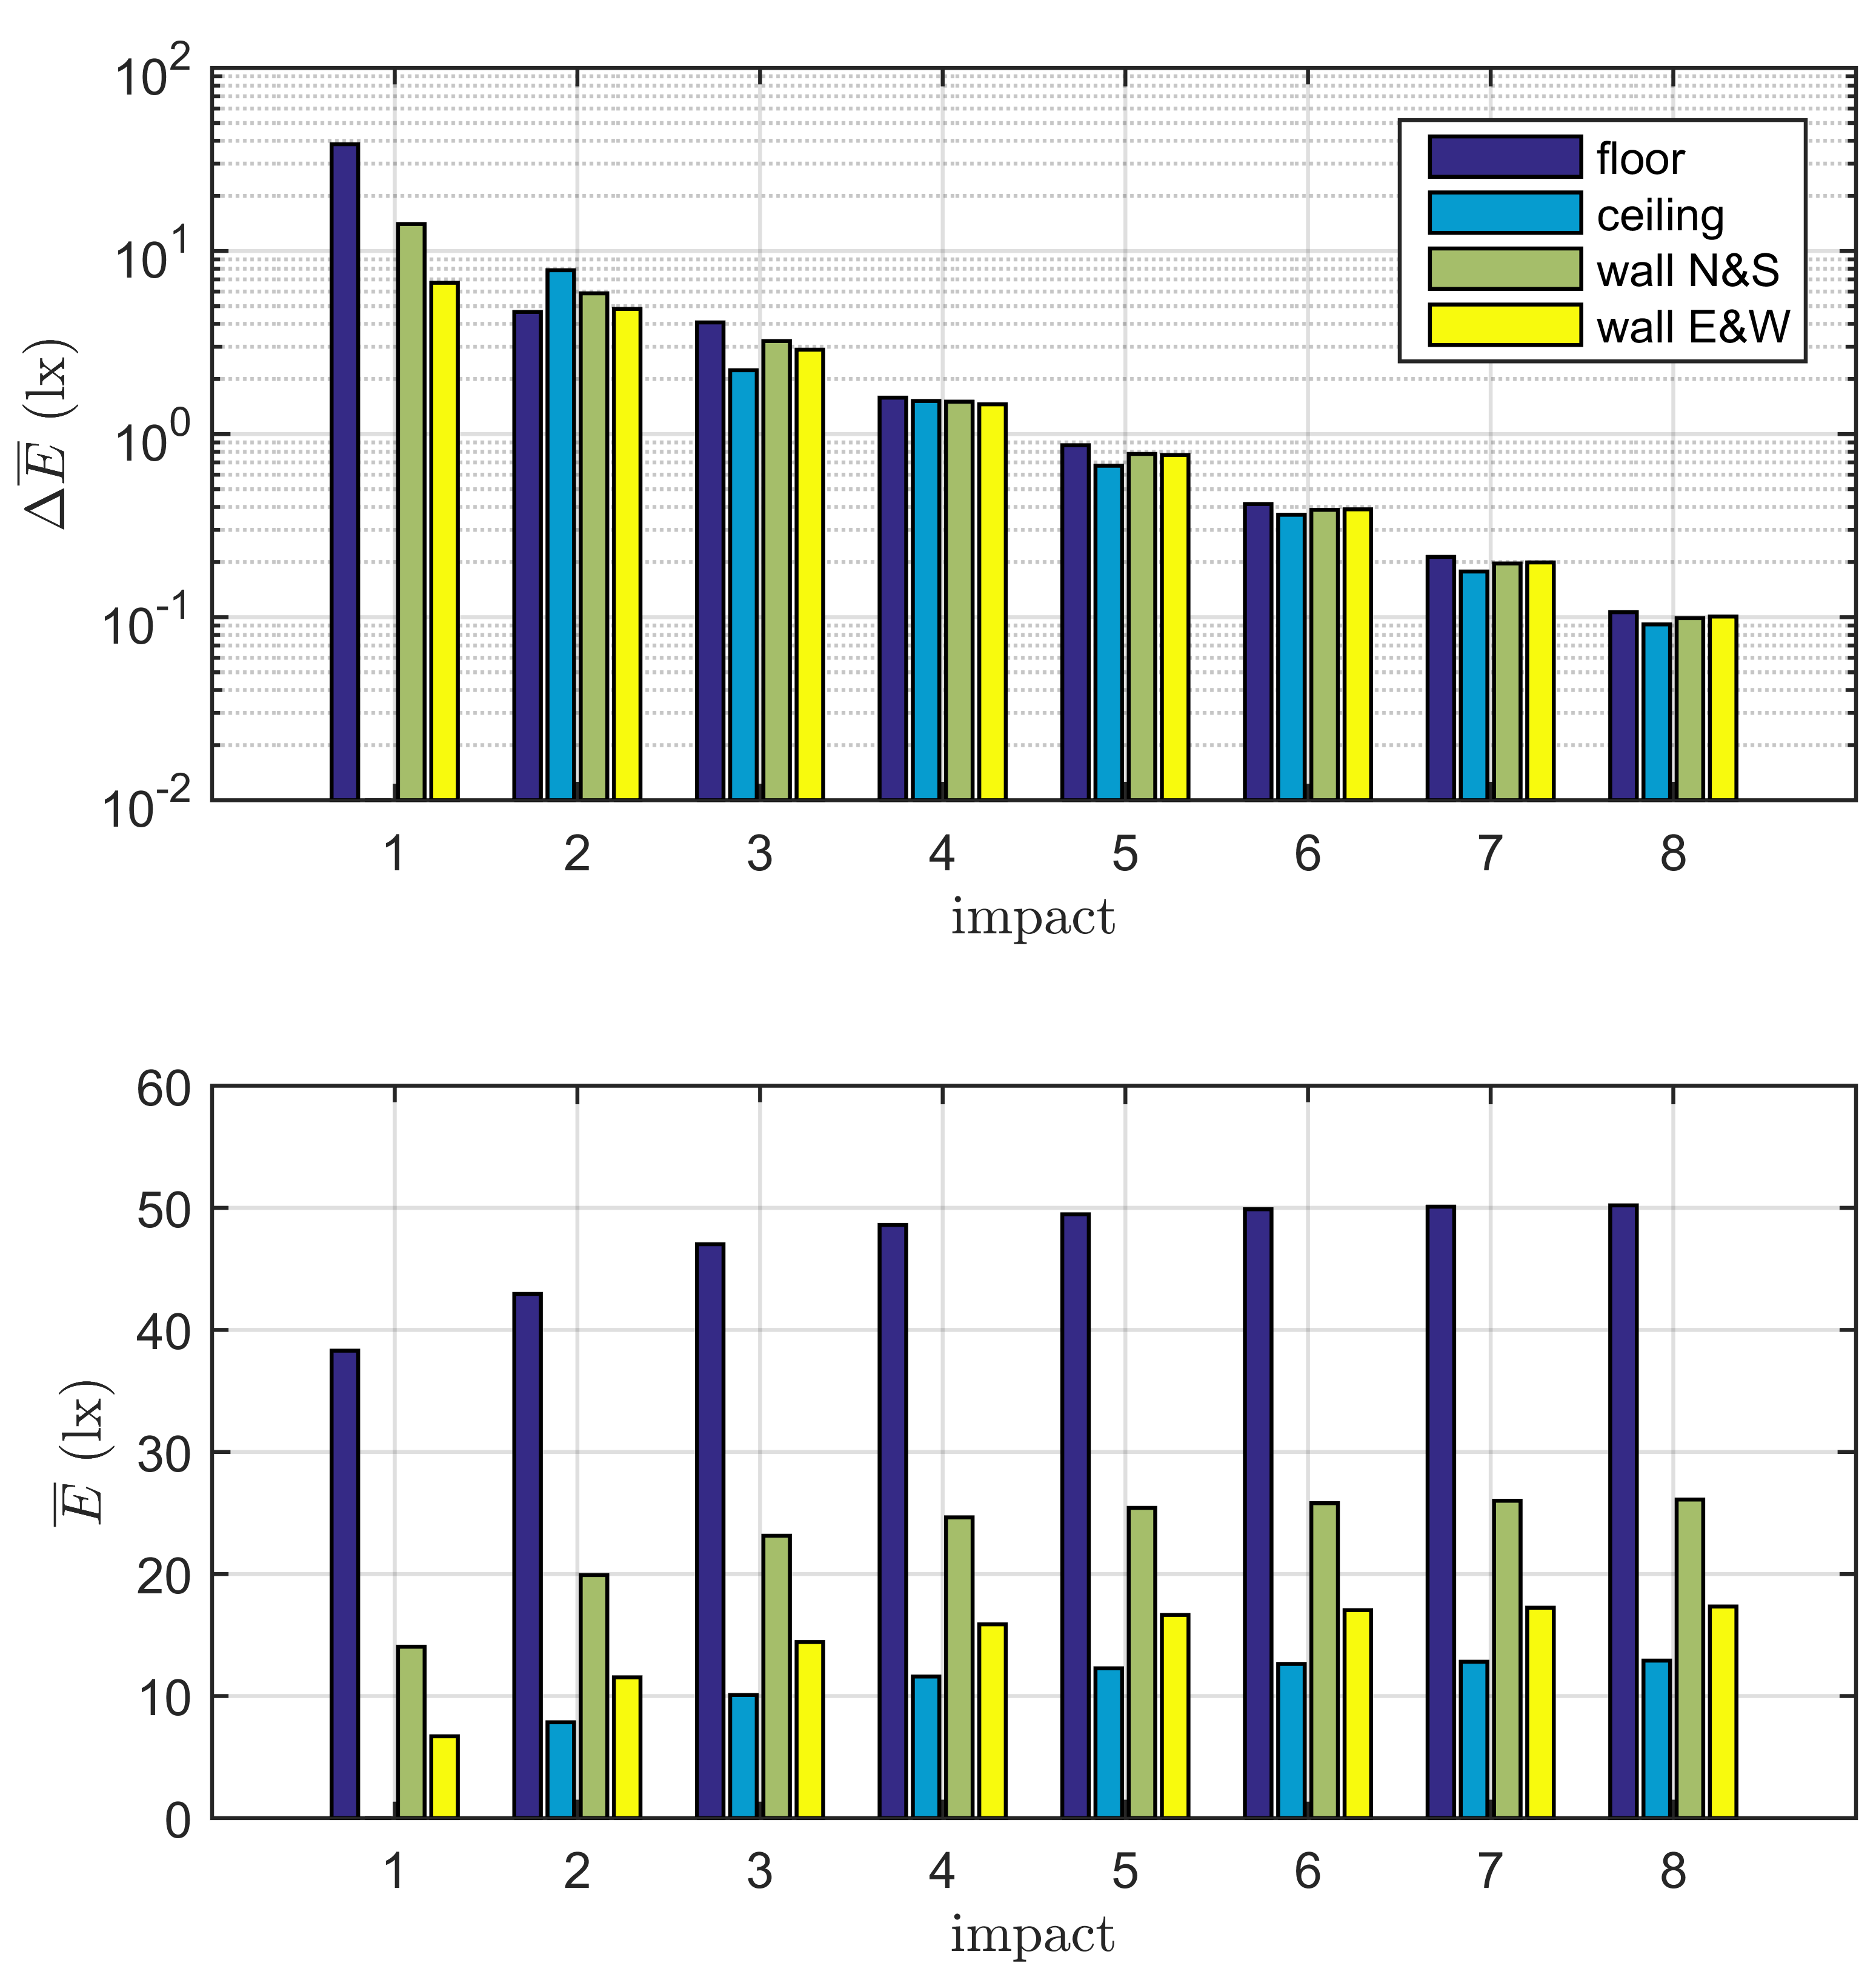
\includegraphics[width=\columnwidth]{reflDif}
  \caption{Increase of the average wall illuminance for one lamp mounted in the center of the room's ceiling depending on the count of light impacts, i.e. number of reflections - 1.}
  \label{fig:reflDif}
\end{figure}

A grid of evenly spaced control points was placed on the reference plane with 25~cm distances between neighboring points. The luminaires were placed in a rectangular area on the ceiling that starts 0.5~m from the eastern and western walls and 0.4~m from the northern and southern walls (Figure~\ref{fig:modRoom}). All further presented results were evaluated for the same luminaire  MSTR~SLB~4x18W. The luminaire's spacial luminous intensity distribution data were taken from the software "Building Design". All placed luminaires were oriented equally with half-planes $C90^\circ$ in direction of $y$-axis as depicted in Figure~\ref{fig:modRoom}. The luminous intensity curve of the used luminaire is shown in Figure~\ref{fig:IDiag}. The considered dimension of the luminaire were 595~mm $\times$ 595~mm $\times$ 80~mm.

\begin{figure}[htb]
  \centering
  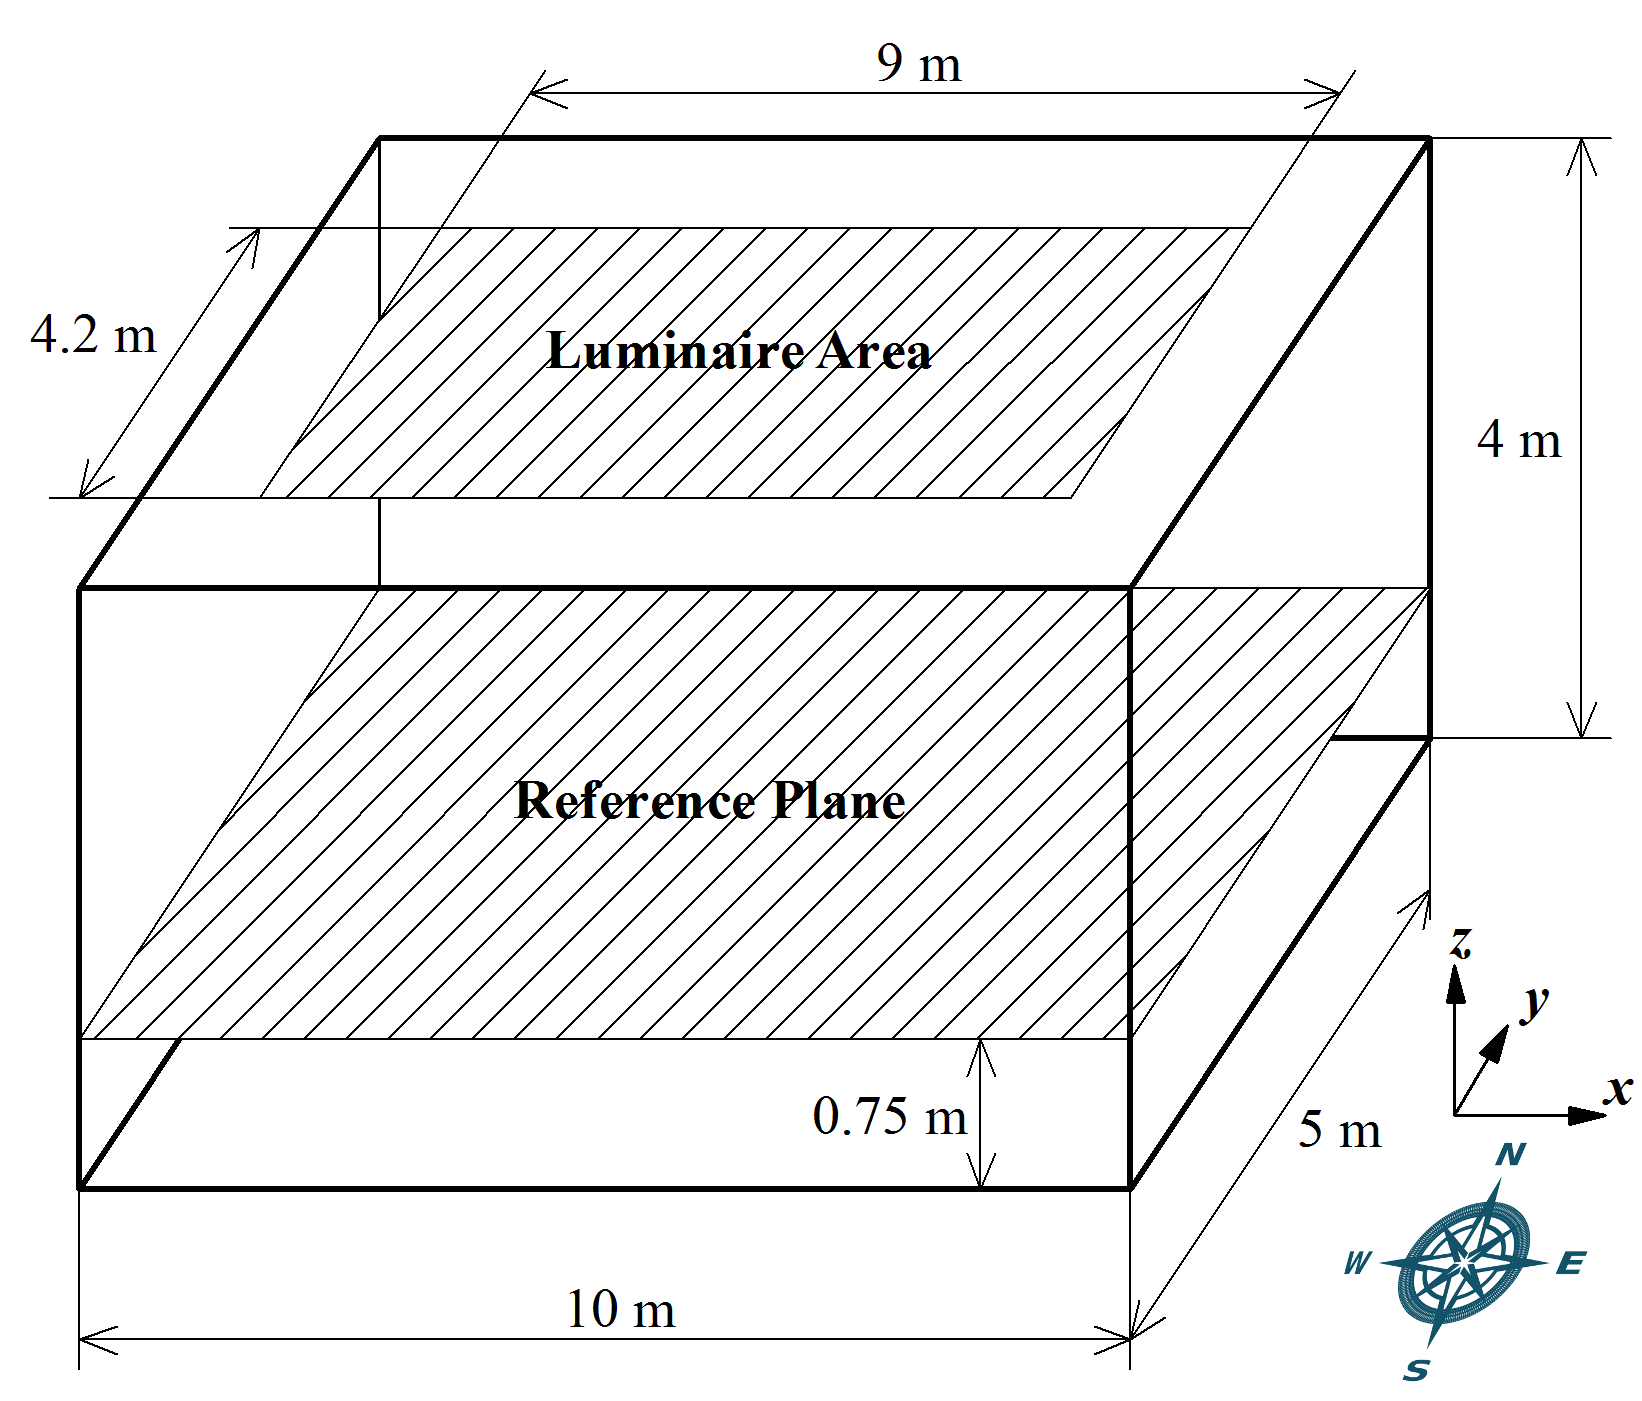
\includegraphics[width=\columnwidth]{modRoom2}
  \caption{Model room dimensions}
  \label{fig:modRoom}
\end{figure}

\begin{figure}[htb]
  \centering
  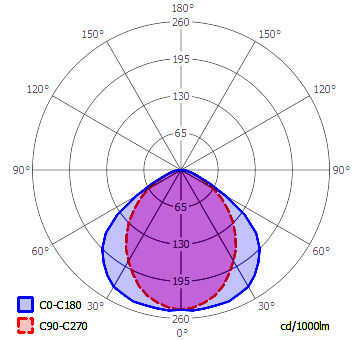
\includegraphics[width=0.8\columnwidth]{IDiag}
  \caption{Luminous intensity distribution curve of the luminaire MSTR SLB 4x18W}
  \label{fig:IDiag}
\end{figure}